\documentclass[11pt, openany, a4paper]{article}

\usepackage{etex}
\usepackage{fullpage}
\usepackage{pstricks,pstricks-add,pst-math,pst-xkey}
\usepackage[frenchb]{babel}
%\usepackage{slashbox}
\usepackage{graphicx}
\usepackage{amsmath,amssymb,amstext,amsthm}
%\usepackage{comment}
\usepackage[utf8]{inputenc}
\usepackage[OT1]{fontenc}
\usepackage{pgf,tikz}
\usepackage{pgfplots}
\usepackage{floatpag}
\usepgfmodule{shapes}
\usetikzlibrary{arrows,patterns}
\usepackage{floatflt}
\usepackage{import}
\usepackage{xcolor}
\usepackage{natbib}
%\usepackage{fourier-orns}

\newcounter{moncompteur}
\newtheorem{q}[moncompteur]{ \textbf{Question}}{}
\newtheorem{prop}[moncompteur]{ \textbf{Proposition}}{}
\newtheorem{df}[moncompteur]{ \textbf{Définition}}{}
\newtheorem*{df*}{ \textbf{Définition}}{}
\newtheorem{rem}[moncompteur]{ \textbf{Remarque}}{}
\newtheorem{theo}[moncompteur]{ \textbf{Théorème}}{}
\newtheorem{conj}[moncompteur]{ \textbf{Conjecture}}{}
\newtheorem{cor}[moncompteur]{ \textbf{Corollaire}}{}
\newtheorem{lm}[moncompteur]{ \textbf{Lemme}}{}
%\newtheorem{nota}[moncompteur]{ \textbf{Notation}}{}
%\newtheorem{conv}[moncompteur]{ \textbf{Convention}}{}
\newtheorem{exa}[moncompteur]{ \textbf{Exemple}}{}
\newtheorem{ex}[moncompteur]{ \textbf{Exercice}}{}
%\newtheorem{app}[moncompteur]{ \textbf{Application}}{}
%\newtheorem{prog}[moncompteur]{ \textbf{Algorithme}}{}
%\newtheorem{hyp}[moncompteur]{ \textbf{Hypothèse}}{}
\newenvironment{dem}{\noindent\textbf{Preuve}\\}{\flushright$\blacksquare$\\}
\newcommand{\cg }{[\kern-0.15em [}
\newcommand{\cd}{]\kern-0.15em]}
\newcommand{\R}{\mathbb{R}}
\newcommand{\K}{\mathbb{K}}
\newcommand{\N}{\mathbb{N}}
\newcommand{\Z}{\mathbb{Z}}
\newcommand{\C}{\mathbb{C}}
\newcommand{\U}{\mathbb{U}}
\newcommand{\Q}{\mathbb{Q}}
\newcommand{\B}{\mathbb{B}}
\newcommand{\card}{\mathrm{card}}
\newcommand{\norm}[1]{\left\lVert#1\right\rVert}
\pgfplotsset{compat=newest}
\newcommand{\La}{\mathcal{L}}
\newcommand{\Ne}{\mathcal{N}}
\newcommand{\D}{\mathcal{D}}
\newcommand{\Ss}{\textsc{safestay}}
\newcommand{\Sg}{\textsc{safego}}
\newcommand{\M}{\textsc{move}}
\newcommand{\E}{\mathcal{E}}
\newcommand{\V}{\mathcal V}
\setlength{\parindent}{0pt}
\newcommand{\myrightleftarrows}[1]{\mathrel{\substack{\xrightarrow{#1} \\[-.6ex] \xleftarrow{#1}}}}
\newcommand{\longrightleftarrows}{\myrightleftarrows{\rule{1cm}{0cm}}}

\definecolor{bleuclair}{rgb}{0.75,0.75,1.0}
\newcommand{\ANNOT}[1]{
  ~\linebreak
  \centerline{
    %{\Huge{\danger}}
    \large\fcolorbox{black}{bleuclair}{
      \begin{minipage}[h]{.8\linewidth}
      #1
      \end{minipage}
    }
    %{\Huge{\danger}}
  }
}

\newcommand\tikzmark[1]{%
  \tikz[overlay,remember picture,baseline] 
  \node[anchor=base](#1){};}

\newcommand\MyLine[3][]{%
  \begin{tikzpicture}[overlay,remember picture]
    \draw[#1] (#2.north west) -- (#3.south east);
  \end{tikzpicture}}


\graphicspath{{.}}
\newcommand{\e}[1]{$\times 10^{#1}$}
\begin{document}

\title{Algorithmes pour les systèmes de recommandation : un comparatif}
\date{}
\maketitle
\section*{Introduction}

Un algorithme de \emph{collaborative filtering} a pour but de se baser sur le comportement passé des utilisateurs pour proposer des recommandations pertinentes. On va ici se placer dans le cadre d'une matrice de ratings donnés par des utilisateurs à des objets, éventuellement incomplète voire parcimonieuse. Étant donné un sous-ensemble des ratings, le but est d'estimer les autres.

On a plusieurs attentes vis-à-vis d'un tel algorithme :
\begin{itemize}
	\item{Requêtes rapides : un utilisateur doit pouvoir obtenir rapidement une recommandation (typiquement, l'objet à qui on estime qu'il attribuera le meilleur score).}
	\item{Ajout d'un nouvel utilisateur : on aimerait pouvoir ajouter raisonnablement vite un nouvel utilisateur à la base de données, en mettant à jour à la volée l'estimation des ratings des autres utilisateurs.}
	\item{Démarrage à froid : on aimerait qu'un utilisateur ayant donné peu de ratings puisse recevoir des recommendations pertinentes.}
	\item{Précision : on cherche à obtenir les recommandations les plus pertinentes possibles.}
\end{itemize}

On peut s'attendre à ce que l'efficacité d'un algorithme varie selon les caractéristiques du jeu de données (forme de la matrice, caractère parcimonieux ou non...)

Dans la suite, nous allons comparer nos implémentations de différents algorithmes de collaborative filtering en terme de précision (au sens de l'erreur MSE) et de temps de calcul (pour fournir une estimation complète des ratings à partir d'une matrice à trous).


\tableofcontents

\section{Les algorithmes utilisés}
	\subsection{Algorithmes témoins}
		Algorithmes simples (voire naïfs pour certains) servant de points de comparaison : 
			\begin{itemize}
				\item{"Witness" : Estimer tous les ratings inconnus par la moyenne de tous les ratings exprimés}
				\item{"PerUserAverage" : Estimer tous les ratings inconnus pour un utilisateur donné par la moyenne des ratings connus qu'il a attribués}
				\item{"BiasFromMean" : Estimer la note donnée par un utilisateur à un objet en fonction de sa moyenne, mais aussi des écarts entre les notes attribuées à l'objet et les moyennes des utilisateurs qui l'ont noté}
				\item{"UnbiasedWitness" : Retirer les biais (cf. \ref{simCos}), estimer tous les ratings inconnus par $0$, remettre les biais}
			\end{itemize}
	
	\subsection{Algorithmes Slope One}
		Prédicteur affine, en imposant une pente de 1. Pour tout couple d'objet, on définit une déviation de l'un par rapport à l'autre, un peu comme la mesure de similarité cosinus, mais en beaucoup plus simple (linéaire). La prédiction de la note attribuée à un objet s'obtient alors en ajoutant la moyenne de l'utilisateur et la moyenne des déviations de l'objet aux autres objets notés par l'utilisateur. D'où un prédicteur de forme $f(x)=x+b$.
	
		
		
		Calculs simples. Possibilité de garder les déviations en mémoire : traitement d'une requête très rapide. De plus, ces déviations peuvent même être mises à jour sans tout recalculer quand on ajoute un rating.
		
		\`A quel point est-ce moins précis que d'autres algos plus sophistiqués ?
		
		Variante : donner plus de poids aux déviations des paires d'objets qui ont été notés tous deux à la fois par un grand nombre d'utilisateurs, car elles sont plus fiables.
		
		Algorithmes tirés de \cite{Lemire2007}.
	\subsection{Algorithmes par similarité cosinus}
		\label{simCos}
		Implémentation des algorithmes vus en cours : on calcule les biais en résolvant le problème d'optimisation $$\min_{b^i, b_j}\sum_{i,j\in\Omega}(r_{ij} - \overline{r} - b^i - b_j)$$ via la solution matricielle du cours, puis on calcule des scores de similarité entre utilisateurs ou entre objets en utilisant le cosinus de l'angle comme mesure de similarité entre deux vecteurs et on estime les ratings comme une moyenne pondérée par les scores de similarité.
		
	\subsection{SVD}
	Variations sur la question bonus du DM $2$. L'algorithme du DM commence par estimer les ratings inconnus à $0$ avant d'appliquer la décomposition en valeurs singulières. L'estimation à 0 permet de faire des calculs sur des matrices creuses quand on connaît peu de ratings, donc un temps de calcul plus court. Les variantes qui suivent opèrent différentes transformations sur la matrice à estimer avant d'appliquer l'algorithme du DM, le but étant que l'estimation à 0 soit aussi pertinente que possible.

		\subsubsection{ShiftSVD} 
		
		On calcule le rating moyen $\overline{r}$, on applique l'algorithme du DM à $R-\overline{r}$ et on ajoute $\overline{r}$ au résultat.
			
		\subsubsection{UnbiasedSVD}
		
		Plutôt que de se contenter de retrancher le rating moyen partout, on calcule les biais en résolvant le problème d'optimisation vu en cours comme en section \ref{simCos}, on applique l'algorithme du DM à la matrice non biaisée puis on réintroduit les biais.
		On s'attend à un résultat plus précis, mais le temps de calcul des biais est non négligeable (il faut inverser une matrice).
		
	\subsection{Analyse en composantes principales : algorithme Eigentaste}
		Idée : s'appuyer sur un petit sous-ensemble d'objets notés par tous les utilisateurs (\emph{gauge set}) pour projeter un utilisateur sur un espace de petite dimension puis estimer ses notes à partir de celles de ses voisins au sens d'un algorithme de clustering. Eigentaste ne s'applique donc qu'aux jeux de données comprenant un tel gauge set, comme le jeu de données Jester. L'algorithme est détaillé dans \cite{Goldberg2001}, nous le reprenons ici.
		
		Notons $R$ la matrice $(n\times m)$ des ratings, $G$ le gauge set, $k=|G|$.
		
		On commence par normaliser les ratings des utilisateurs sur les objets du gauge set : la qualité objective d'un objet importe peu ici car on cherche à obtenir des informations sur les ressemblances entre utilisateurs par analyse de composantes principales.
		
		Pour tout objet $j$, on calcule donc $\mu_j=\sum_{i=1}^n r_{ij}$ la note moyenne de cet objet, et $$\sigma_j^2 = \frac{1}{n-1} \sum_{i=1}^{n} (r_{ij} - \mu_j)$$ sa variance.
		
		On obtient alors la matrice $A$ (de taille $k\times k$) des ratings normalisés sur le gauge set : $a_{ij} = \frac{r_{ij}-\mu_j}{\sigma_j}$.
		
		On pose $C=\frac{1}{n-1} A^T A$ (matrice de corrélation de Pearson). Elle est symétrique définie positive, on note $\Lambda$ la matrice diagonale contenant ses valeurs propres triées par ordre décroissant et $E$ la matrice orthogonale de vecteurs propres associée. On a $EE^T = Id$, $C = E\Lambda E^T$.
		
		On peut alors projeter les vecteurs correspondant aux utilisateurs sur un petit sous-espace (de dimension $v$) contenant l'essentiel de la variance en posant $X=AE^T_v$. 
		En particulier, pour $v=k$, on a $C_X = \frac{1}{n-1} X^T X = ECE^T = \Lambda$ diagonale : les vecteurs sont décorrélés.
		On prend $v=2$ dans la suite.
		
			\begin{figure}[ht!]
				\centering
				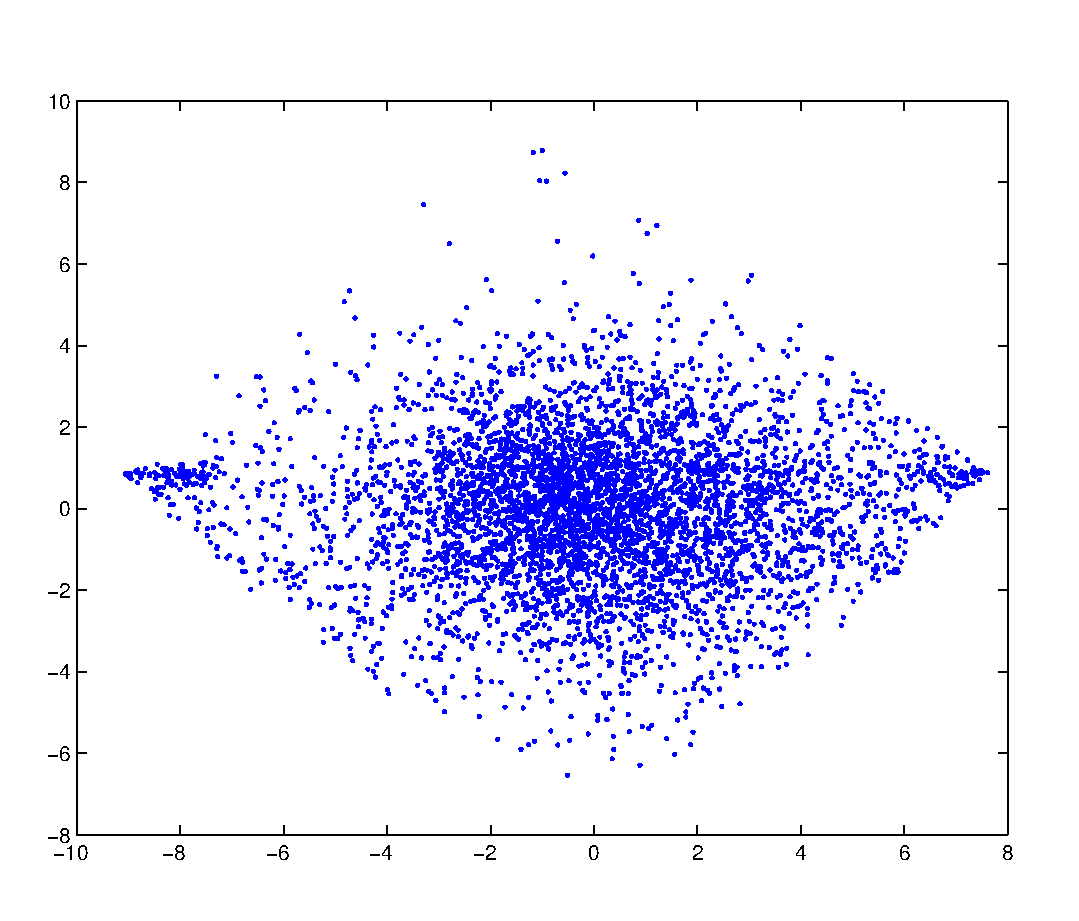
\includegraphics[height=120mm]{eigentaste_proj_cropped.pdf}
				\caption{Projection pour $v=2$ sur un sous-ensemble du jeu de données Jester}
			\end{figure}
			
		On regroupe ensuite les utilisateurs proches par amas en utilisant un algorithme de clustering (\cite{Goldberg2001} utilise un algorithme récursif rectangulaire, nous avons utilisé les fonctions Matlab \emph{linkage} et \emph{cluster} dans notre implémentation).
		
		On estime ensuite un rating de l'utilisateur $i$ sur l'objet $j$ par la moyenne des notes pour $j$ des utilisateurs se trouvant dans le même cluster que $i$.
		
		\medskip
						
		Cet algorithme a l'inconvénient de ne s'appliquer qu'à certains jeux de données : pour ajouter un nouvel utilisateur, il faut d'abord lui faire noter l'intégralité du gauge set (typiquement une dizaine d'objets). De plus, on ne peut rien dire sur un utilisateur seul dans son amas : le démarrage à froid pose problème.
		
		En revanche, ajouter un utilisateur qui a noté le gauge set est peu coûteux en termes de temps de calcul : on peut lui recommander rapidement des objets dès qu'on a choisi son cluster, l'idée étant de ne pas modifier immédiatement les projections des anciens utilisateurs mais plutôt de tout remettre à jour périodiquement.
		
		Dans la suite, on se propose de comparer Eigentaste avec d'autres algorithmes de recommandation en termes de précision et de temps de calcul, sur le jeu de données Jester (pour lequel Eigentaste a été mis au point).
		
		
		
		
\section{Observations expérimentales}
	\subsection{Jeux de données}
	\subsubsection{La matrice du DM}
		
		Il s'agit d'une matrice pleine, de taille $100 \times 1000$ et de rang $10$, dont les coefficients sont des réels entre $0$ et $1$. Pour évaluer un algorithme, on fixe une probabilité $p$, on fournit à l'algorithme une sous-matrice dans laquelle chaque rating est présent avec probabilité $p$ (de façon indépendante des autres), on s'en sert pour calculer une matrice pleine qu'on compare avec la matrice de départ.
		
		On peut tester sur cette matrice tous les algorithmes présentés sauf Eigentaste (pas de gauge set).
		
	\subsubsection{Le jeu de données Jester}
		Jeu de données mis à disposition par Ken Goldberg (Berkeley). Il s'agit de ratings d'une centaine de blagues par de nombreux utilisateurs (plus de $50 000$). Huit blagues ont été notées par tous les utilisateurs : on s'en sert comme gauge test pour implémenter Eigentaste. Les coefficients varient continûment de $-10$ à $10$ : on les ramène à $[0,1]$ par une transformation affine pour mieux comparer avec la matrice du DM.
		
		La densité $d$ de la matrice est d'environ $0.24$. Pour $p<d$, on conserve une proportion $p/d$ des coefficients aléatoirement : on obtient à nouveau une matrice de densité $p$ pour pouvoir comparer avec le jeu de données précédent.
		
		Comme le rang de la matrice cible est inconnu (elle n'est pas pleine) les algorithmes à base de SVD donnent d'assez mauvais résultats (en ne tronquant pas du tout la décomposition en valeurs singulières).
		
		Contrairement à la matrice du DM, les objets notés par les utilisateurs ne sont pas choisis au hasard : il s'agit de recommandations qu'on leur a faites après qu'ils ont noté le gauge set, ils ont donc plutôt tendance à noter des objets qu'ils apprécient.
		
		Par ailleurs, la forme de la matrice est inversée par rapport à celle du DM : il y a beaucoup d'utilisateurs et très peu d'objets.
		
		Pour avoir des temps de calcul et des utilisations mémoire raisonnables sur nos machines personnelles, nous nous sommes restreints aux $5000$ premiers utilisateurs.
	
	\subsection{Mesures d'erreur}
	
		\begin{figure}[ht!]
			\centering
			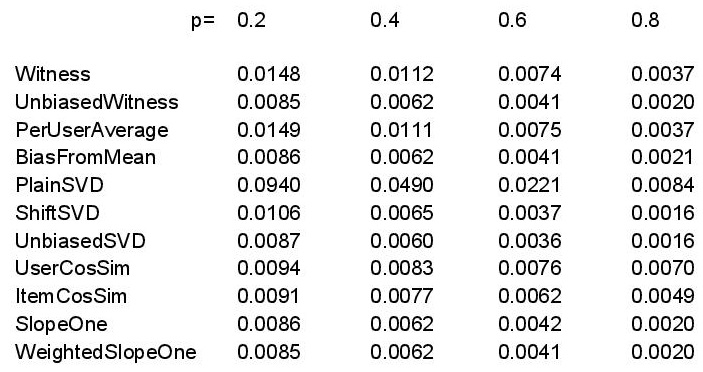
\includegraphics[width=0.8\linewidth]{resultatsPrerapport.jpg}
		\end{figure}
		Sur la matrice du DM, on obtient ce tableau d'erreurs MSE pour différentes valeurs de p :
		
		
		Les algorithmes simples "BiasFromMean" et "UnbiasedWitness" obtient d'excellents résultats ! Les variantes de Slope One obtiennent aussi des résultats très comparables à l'algorithme UnbiasedSVD plus complexe à mettre en œuvre.
		
		On observe que sur la matrice du DM, il est préférable de considérer la similarité par utilisateur, alors que pour le jeu de données Jester, il vaut mieux utiliser la similarité par objet : c'est très probablement lié au fait que dans le jeu de données Jester, il y a beaucoup plus d'utilisateurs que d'objets alors que c'est l'inverse dans la matrice du DM.
		
	\subsection{Choix des paramètres pour Eigentaste}
	
		L'algorithme de clustering utilisé dans le calcul de Eigentaste prend un paramètre qu'il faut optimiser pour augmenter la précision : le nombre maximal de clusters. On observe que le nombre optimal de clusters varie fortement avec $p$ : pour $p=0.2$, il faut en prendre environ $600$ (pour classifier $5000$ utilisateurs), alors que pour $p=0.1$, il est préférable de n'en prendre qu'une vingtaine (voir Figure \ref{clusterfig}). Ceci est probablement lié à un phénomène de surapprentissage : quand $p$ est petit, on n'a pas assez d'informations pour justifier de séparer certains utilisateurs.
		
		\begin{figure}[ht!]
			\centering
			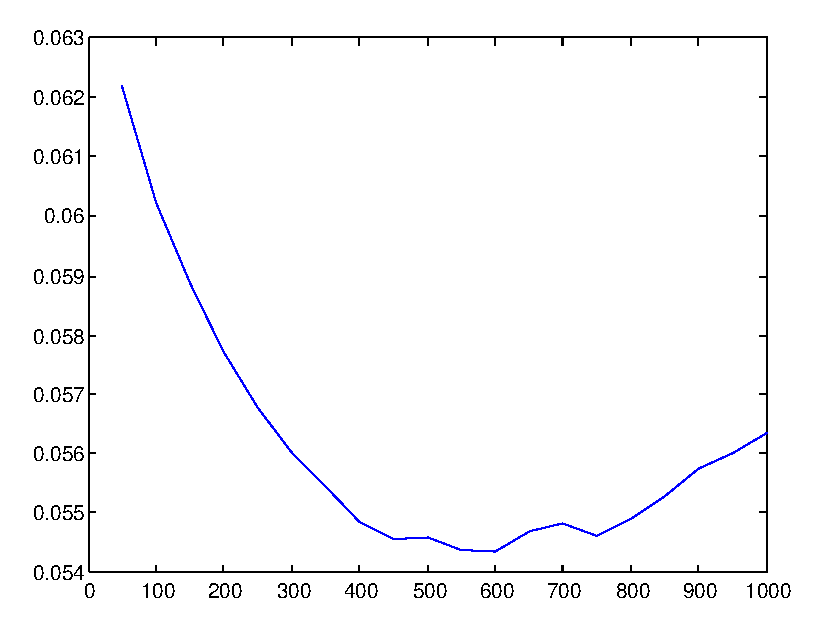
\includegraphics[height=120mm]{optimalMaxClust01_cropped.pdf}
			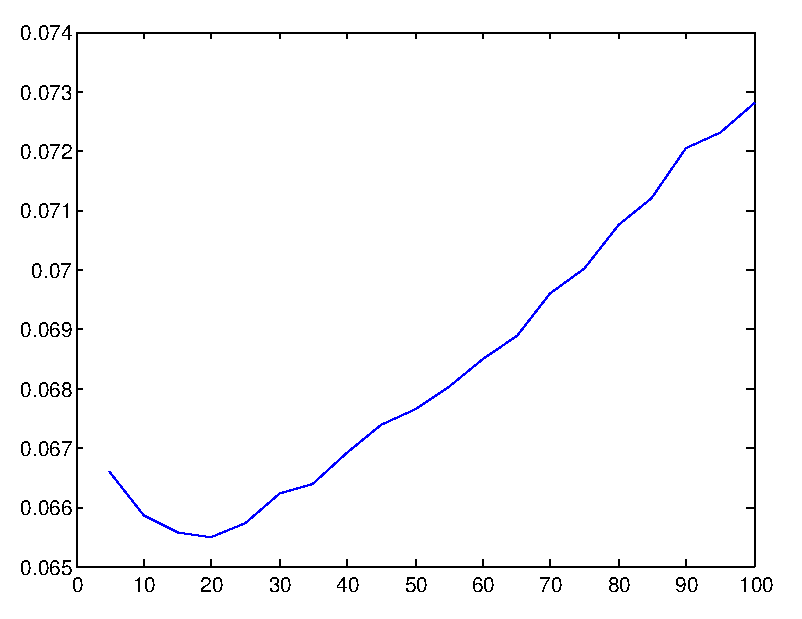
\includegraphics[height=120mm]{optimalMaxClust02_cropped.pdf}
			\caption{Erreur MSE en fonction du nombre maximal de clusters pour $p=0.2$ et $p=0.1$}
			\label{clusterfig}
		\end{figure}
		
	\subsection{Temps d'exécution}
	
		\begin{figure}[ht!]
			\centering
			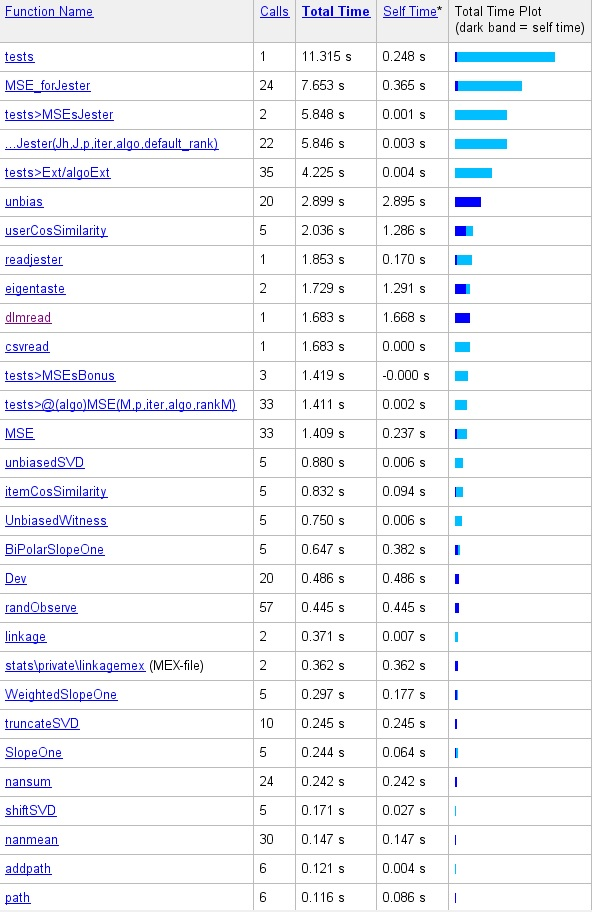
\includegraphics[height=120mm]{times.jpg}
			\caption{Profiling fourni par Matlab}
		\end{figure}
		

		Une bonne partie du temps de calcul est passé à inverser des matrices presque singulières pour calculer les biais... Ainsi, l'algorithme UnbiasedWitness, qui est très simple conceptuellement et parmi les plus précis sur les deux jeux de données, est loin d'être le moins coûteux en terme de temps de calcul.
				
		Il faut aussi tenir compte du fait que certains algorithmes (tels que Slope One ou Eigentaste, mais pas les variantes de SVD) font beaucoup de calculs "une fois pour toutes" (\emph{off-line}). Une fois ces calculs faits, les requêtes et l'ajout d'un nouvel utilisateur sont rapides. 
		
\bibliographystyle{plain}
\bibliography{biblio}

\end{document}